% !TEX TS-program = XeLaTeX
% use the following command:
% all document files must be coded in UTF-8
\documentclass[english]{textolivre}
% build HTML with: make4ht -e build.lua -c textolivre.cfg -x -u article "fn-in,svg,pic-align"

\journalname{Texto Livre}
\thevolume{15}
\theyear{2022}
\receiveddate{\DTMdisplaydate{2021}{7}{29}{-1}} % YYYY MM DD
\accepteddate{\DTMdisplaydate{2021}{10}{18}{-1}}
\publisheddate{\DTMdisplaydate{2022}{1}{27}{-1}}
\corrauthor{Cláudia Aparecida Fonseca}
\articledoi{10.35699/1983-3652.2022.35445}
%\articleid{NNNN} % if the article ID is not the last 5 numbers of its DOI, provide it using \articleid{} commmand
\runningauthor{Fonseca et al.} 
%\editorname{Leonardo Araújo} % old template
\sectioneditorname{Daniervelin Pereira}
\layouteditorname{Daniervelin Pereira}

\title{Representation of structured data of the text genre as a technique for automatic text processing}
\othertitle{Representação dos dados estruturados do gênero textual como técnica para o processamento automático de texto}
% if there is a third language title, add here:
%\othertitle{Artikelvorlage zur Einreichung beim Texto Livre Journal}

\author[1]{Claudia Aparecida Fonseca~\orcid{0000-0003-1945-0872}~\thanks{Email: \url{claudia.fonseca@ufvjm.edu.br}}}
\author[2]{Marcus Vinícius Carvalho Guelpeli~\orcid{0000-0001-5724-1081}~\thanks{Email: \url{marcus.guelpeli@ufvjm.edu.br}}}
\author[3]{Rafael Santiago de Souza Netto~\orcid{0000-0003-1231-5387}~\thanks{Email: \url{rafael.santiago@tutanota.com}}}
\affil[1]{Universidade Federal dos Vales do Jequitinhonha e Mucuri, Departamento de Letras, Diamantina, MG, Brasil.}
\affil[2]{Universidade Federal dos Vales do Jequitinhonha e Mucuri, Departamento de sistema de informação, Diamantina, MG, Brasil.}
\affil[3]{Centro Universitário de Barra Mansa, Departamento de Ciência da Computação, Barra Mansa, RJ, Brasil.}

\addbibresource{article.bib}
% use biber instead of bibtex
% $ biber article

% used to create dummy text for the template file
\definecolor{dark-gray}{gray}{0.35} % color used to display dummy texts
\usepackage{lipsum}
\SetLipsumParListSurrounders{\colorlet{oldcolor}{.}\color{dark-gray}}{\color{oldcolor}}

% used here only to provide the XeLaTeX and BibTeX logos
\usepackage{hologo}

% if you use multirows in a table, include the multirow package
\usepackage{multirow}

% provides sidewaysfigure environment
\usepackage{rotating}

% CUSTOM EPIGRAPH - BEGIN 
%%% https://tex.stackexchange.com/questions/193178/specific-epigraph-style
\usepackage{epigraph}
\renewcommand\textflush{flushright}
\makeatletter
\newlength\epitextskip
\pretocmd{\@epitext}{\em}{}{}
\apptocmd{\@epitext}{\em}{}{}
\patchcmd{\epigraph}{\@epitext{#1}\\}{\@epitext{#1}\\[\epitextskip]}{}{}
\makeatother
\setlength\epigraphrule{0pt}
\setlength\epitextskip{0.5ex}
\setlength\epigraphwidth{.7\textwidth}
% CUSTOM EPIGRAPH - END

% LANGUAGE - BEGIN
% ARABIC
% for languages that use special fonts, you must provide the typeface that will be used
% \setotherlanguage{arabic}
% \newfontfamily\arabicfont[Script=Arabic]{Amiri}
% \newfontfamily\arabicfontsf[Script=Arabic]{Amiri}
% \newfontfamily\arabicfonttt[Script=Arabic]{Amiri}
%
% in the article, to add arabic text use: \textlang{arabic}{ ... }
%
% RUSSIAN
% for russian text we also need to define fonts with support for Cyrillic script
% \usepackage{fontspec}
% \setotherlanguage{russian}
% \newfontfamily\cyrillicfont{Times New Roman}
% \newfontfamily\cyrillicfontsf{Times New Roman}[Script=Cyrillic]
% \newfontfamily\cyrillicfonttt{Times New Roman}[Script=Cyrillic]
%
% in the text use \begin{russian} ... \end{russian}
% LANGUAGE - END

% EMOJIS - BEGIN
% to use emoticons in your manuscript
% https://stackoverflow.com/questions/190145/how-to-insert-emoticons-in-latex/57076064
% using font Symbola, which has full support
% the font may be downloaded at:
% https://dn-works.com/ufas/
% add to preamble:
% \newfontfamily\Symbola{Symbola}
% in the text use:
% {\Symbola }
% EMOJIS - END

% LABEL REFERENCE TO DESCRIPTIVE LIST - BEGIN
% reference itens in a descriptive list using their labels instead of numbers
% insert the code below in the preambule:
%\makeatletter
%\let\orgdescriptionlabel\descriptionlabel
%\renewcommand*{\descriptionlabel}[1]{%
%  \let\orglabel\label
%  \let\label\@gobble
%  \phantomsection
%  \edef\@currentlabel{#1\unskip}%
%  \let\label\orglabel
%  \orgdescriptionlabel{#1}%
%}
%\makeatother
%
% in your document, use as illustraded here:
%\begin{description}
%  \item[first\label{itm1}] this is only an example;
%  % ...  add more items
%\end{description}
% LABEL REFERENCE TO DESCRIPTIVE LIST - END


% add line numbers for submission
%\usepackage{lineno}
%\linenumbers

\usepackage{needspace}
\usepackage[htt]{hyphenat}

\begin{document}
\maketitle

\begin{polyabstract}
\begin{abstract}
The present article was developed in the field of Natural Language Processing and Language Studies based on a corpus compiled by computational tools. This study is based on the assumption that it is helpful to trace a close relationship between corpus generation/annotation and the assessment of the constitutive elements of the text genre source. It aims to demonstrate, through specific studies of structured data from the text genre ‘scientific article’, alternatives to automatic text processing techniques. In order to reach the intended goal, the authors created a computational model for the compilation of a linguistic, specialized Corpus, representative of the genre Scientific Article - CorpACE. The object of study includes the constitutive elements of scientific articles, marked in XML, extracted and collected from the SciELO-Scientific Electronic Library On-line database. The final product was a database obtained with information extracted and structured in XML format, which designates and identifies the markups of the genre being analyzed and is available for many tools and applications. The results demonstrate how the representation of constitutive elements of the genre can condense available information with hierarchical and dynamic processes built during the compilation. At the end of the study, it is believed that more research will be required for bringing Language Science and Computer Science closer with emphasis on NLP in the attempt to represent and manipulate linguistic knowledge in its many levels – morphological, syntactic, semantic and discursive – in order to improve implementation and manipulation of automatic text processing.

\keywords{\textit{Corpus} linguistics \sep Natural language processing \sep Scientific article \sep Text genre \sep \textit{Corpora} annotation}
\end{abstract}

\begin{portuguese}
\begin{abstract}
O presente trabalho foi desenvolvido na área de Processamento de Linguagem Natural (PLN) e Estudos Linguísticos baseados em \textit{corpus} compilado por ferramentas computacionais. Este trabalho parte do princípio de que é necessário assinalar uma estreita relação entre anotação e geração de \textit{corpus} com a análise dos elementos constitutivos do gênero do texto-base. A proposta visa demonstrar, por via específica do estudo dos dados estruturados do gênero textual artigo científico, uma opção de técnica de processamento automático de texto. Para alcançar os objetivos propostos, criou-se um modelo computacional necessário para a compilação de um \textit{corpus} linguístico, especializado, representativo do gênero Artigo Científico - \textit{CorpACE}. O projeto teve como objeto de estudo os elementos constitutivos do gênero textual artigo científico, marcados em XML, extraídos e coletados do banco de dados da SciELO-\textit{Scientific Electronic Library On-line}. Como produto final, obteve-se uma base de dados com as informações extraídas e estruturadas no formato XML, que delimitam e identificam as marcações do gênero em análise, disponível para várias ferramentas e aplicações. Os resultados demonstram como a representação dos elementos constitutivos do gênero pode condensar as informações disponíveis de forma hierarquizada e dinâmica, construídas durante a compilação. Ao final da pesquisa, presume-se que se fazem necessárias mais pesquisas que aproximem a Ciência da Linguagem da Ciência da Computação com ênfase em PLN na tentativa de representar e manipular os conhecimentos linguísticos em seus vários níveis morfológico, sintático, semântico e discursivo, para a melhoria na implementação e manipulação do processamento automático do texto.

\keywords{Linguística de \textit{corpus} \sep Processamento de linguagem natural \sep Artigo científico \sep Gênero textual \sep Anotação de \textit{corpora}}
\end{abstract}
\end{portuguese}
% if there is another abstract, insert it here using the same scheme
\end{polyabstract}

\section{Introduction}\label{sec-intro}
After the computer and media revolution, electronic documents have become one of the most read scholarly and informational media for much of the world’s population due to widespread internet use. Thousands of electronic documents are being produced and published online every day. However, an enormous amount of information is available mainly in unstructured format; i.e., it is produced for human consumption and thus does not necessarily undergo machine processing \cite{cambria_jumping_2014}. Since the purpose of storing information is its future retrieval, the query will always be formulated according to the user’s need for information.

In order to make full use of these documents online, it is imperative to be able to locate and extract the essence of the information content of these files. However, due to the overwhelming flow of available documents, especially in the academic milieu, it is impossible to read all the retrieved texts, since a person’s reachability is limited and requires plenty of time and effort. An alternative that has been investigated to remedy this limitation is automatic text processing, which involves a set of computational techniques for the analysis and representation of human language \cite{cambria_jumping_2014}.

Automatic Text Processing is an activity generated by technological innovation and the human need for access to information. This means that technology is meant to broaden natural communication between individuals who use natural language through verbal (language) and nonverbal (gestures, images, etc.) codes. This study is interesting, not only from a practical point of view – as it helps the user employ computer tools to access, retrieve and use increasing amounts of information online – but also from a scientific-theoretical point of view, since it requires deep understanding of natural language by machines. This knowledge is associated with processes such as reading, comprehension, presentation, evaluation and production of texts.

Furthermore, it is noteworthy that the access and retrieval of information currently follow algorithmic rules that depend mainly on the textual representation of web pages. This means that these algorithmic rules are efficient in performing tasks such as text retrieval by splitting them into pieces, spell-checking, and word counting. However, when it comes to interpreting sentences and extracting meaningful information from them, their abilities are still very limited.

In addition to that, from a linguistic point of view, the process offers many challenges, such as finding solutions on how to reformulate and combine text fragments to generate a cohesive and coherent discourse \cite{jones_automatic_2007}. That is, language cannot be understood merely as the representation of grammar and language rules, since it manifests itself in a myriad of forms, levels and modalities. Besides semantic and morpho-syntactic aspects, verbal language involves discourse processes that can transmit information about, for instance, time and space. All of this creates a challenge for fields of knowledge such as Language Science and Computer Science with an emphasis on NLP, in order to create standardized representations for metadata that need to be normalized and standardized in a format that the computer can understand.

Deciding to face these challenges, the authors of this work present a computational model for the field of NLP, with an interface with Corpus Linguistics (CL), supported by the compilation and annotation of metadata in the corpus\footnote{The prefix “meta” derives from the Greek word for “beyond”. Metadata is described as information that adds data and whose objective is to render information organization and retrieval easier in databases.  There are many definitions of the term metadata. Literally, it means information about data, and the simplest, most commonly referred description is the datum of data \cite{kucuk_application_2000}.} using concepts of Textual Linguistics (TL), which is able to filter structured resources of the text genre – in this case, scientific articles – as a NLP method. The proposed computational model paired with a corpus compilation is considered to be useful for both scientific purposes, as it explores the nature of linguistic communication, and practical purposes, as it facilitates an effective interaction between man and machine. This type of knowledge can then be used by researchers to develop new pedagogical strategies for the use and application of structured language resources.

\section{Natural Language Processing}\label{sec-normas}
Among other definitions, natural language can be defined as one of the “most flexible and plastic cognitive faculties adaptable to behavioral changes and responsible for the dissemination of the constant social, political and cultural transformations generated by human creativity” \cite[p. 7]{marcuschi_generos_2004}. Thus, it is through natural language that individuals are able to communicate using a set of verbal and nonverbal symbols and signs. For this reason, it is important to emphasize that the meaning of natural language is always related to the situation of use and cannot be dissociated from who uses it or how it is used.

This study adopts the expression \textit{natural language} when referring to the term natural tongue, since the tongue is more susceptible to study and systematization in relation to language, which involves more complex aspects such like perception, intelligence, consciousness and variables such like domain related to social life, among others. Natural language, in a way, means the opposite of artificial language or computer programming. Artificial language is totally context-sensitive, and its rules are defined by a meta-language used to express context-free grammar; in other words, is, a formal way of describing languages through a set of communication instructions and protocols. Moreover, a natural text, i.e., a human-produced text, is understood to be something that exists and circulates in some social environment and has not been created with the sole purpose of composing a study corpus. In this context, the natural language is full of rules, variations and ambiguities, which depend on the analysis of the context of production and circulation, among other aspects, in order to be machine-processed.

In this sense, NLP faces the challenge of developing computer systems that are able to understand human language according to the parameters of a formal language, systematized with well-defined objectives regarding its use. For this reason, in a highly technological age such as the one we are experiencing, it is necessary to improve the linguistic characteristics of software for communication between men and machine to be more efficient.

In order to meet this challenge, NLP needed to involve and unify different areas and create an interdisciplinary understanding that would be able to address and include multiple fields of knowledge, such as: Computer Engineering, which provides methods for illustrating models, to create algorithms, and to develop software; Linguistics, which deals with studying the characteristics of human language and categorizing linguistic forms and practices; Mathematics, which provides formal models and methods, using logic for problem solving and developing theses and hypotheses; Psychology, which studies models and theories that motivate human behavior and its mental processes; Statistics, which offers procedures for predicting measurements based on sample records; and Biology, which is embedded in the underlying architecture of linguistic processes in the human brain \cite{manaris_natural_1998}.

By combining this set of knowledge, albeit from distinct fields, systems of natural language generation are able to convert information from computer databases into a language that is comprehensible to human beings and systems of natural language comprehension convert occurrences of human language into more formal representations, which can be more easily manipulated by computer programs. In this sense, \textcite{Silva_2006} warns that the precursors of NLP studies have already indicated that a computer cannot emulate human language satisfactorily if it is not able to understand the context of the subject under discussion. In order for this to occur, the program would be required to provide a detailed model of the specific domain of the given discourse. This argument converges with the principles of the present study, in viewing the text genre annotation as a relevant tool when implementing NLP systems. To corroborate, \textcite{Silva_2006}, states that it is crucial that:

\begin{quote}
    Emulating aspects of natural language implies equipping a NLP system with various knowledge systems and having it emulate a range of cognitive activities: - having a “simple model of its own mindset”; - having a “detailed model of the discourse’s specific domain”; having a model that represents “morphological, syntactic, semantic and contextual information as well as knowledge of the physical world”; - “understanding the subject under discussion”; - “remembering, discussing, executing plans and actions”; - participating in dialogue by responding, with actions and phrases, to the phrases typed by the user; - asking for clarification when its heuristic programs are unable to understand a sentence. \cite[p. 122]{Silva_2006}
\end{quote}

Ever since its inception in 1950, research in NLP has been devoted mainly to the tasks of machine translation, information retrieval, text summarization, topic modeling and, more recently, opinion mining \cite{cambria_jumping_2014}. In general, NLP is directly concerned with the study of natural language aimed at building specialized software. Thus, its implementation requires several complex subsystems in order to represent several language aspects such as sounds, words, sentences and speech at the most wide-ranging structural levels of meaning and use \cite{vieira_linguistica_2001}. Despite many advances in the field, there is still no software able to combine all approaches and generate a knowledge base that can store information describing the language resources needed for developing NLP application efficiently. This is due to the complexity, wealth of detail and variations of human language, which are hardly adequate to computer formats.

Currently, the NLP study uses techniques and linguistic approaches to corpora annotation using three major levels of analysis: morphological, syntactic and semantic. However, these three main approaches fail to address the complexity of language features that need to be normalized, standardized and transformed into markup language. In this sense, moreover, a pragmatic analysis of language resources must be conducted, as has already been suggested \cite{jones_probabilistic_2000}. The development of a useful NLP system requires a methodological approach to the context of production and circulation of both the base text (input text) and the machine-generated text (output text).

\subsection{Main NLP techniques}\label{sec-conduta}
Based on the assumption of studies that have already been completed on the approach, NLP techniques can be categorized into three classes, namely: statistical, linguistic and hybrid \cite{bharti_automatic_2017}. Among the main NLP techniques and approaches directed to text processing; i.e., which can be used in corpus annotators, a breakdown of the main ones is shown in \Cref{tbl01} highlighting four major levels of linguistic analysis: morphological, syntactic, semantic and discursive:

%\begin{table}[htbp]
\setlength\LTleft{-1in}
\setlength\LTright{-1in}
\begin{longtable}{p{3cm}p{2cm}p{7cm}p{3.5cm}}
\caption{Principais Técnicas em PLN.}\label{tbl01}
%\begin{tabular}{p{2cm}p{2cm}p{6.5cm}p{2.3cm}}
\\
\toprule
\textbf{Technique} & \textbf{Approach} & \textbf{Description} & \textbf{Publications}\\
\hline \\
\endfirsthead
{\footnotesize Removal of \textbf{stopwords} – – (filter)} & {\footnotesize Linguistic} & {\footnotesize Filtering process for removing words with little relevance, in the attempt to measure all the information that does not constitute knowledge in the text. The idea behind this filter is to remove words that contain little or no content, such as articles, prepositions, pronouns, conjunctions, adverbs, numerals and interjections. Additionally, terms that commonly or rarely appear are probably not significantly relevant and thus can also be removed.} & {\footnotesize \textcite{luhn_automatic_1958, salton_introduction_1983, frakes_information_1992,lui_evaluation_2007, de_oliveira_junior_monitoramento_2012}}. \\
\\
{\footnotesize \textbf{TF-IDF} – (Term Frequency – Inverse Document Frequency)} & {\footnotesize Statistical} & {\footnotesize Term Frequency (TF) is based on the premise that the importance of a term appearing in a document is directly proportional to its occurrence. Inverse Document Frequency (IDF) is based on the premise that the specificity of a term can be measured by an inverse function of the number of documents in which it occurs. Therefore, this technique consists in weighing the importance of each term within a background corpus, normally consisting of documents belonging to the same domain and then eliminating the list of very common words.} & {\footnotesize \textcite{luhn_automatic_1958,jones_thesauric_1972,bhatia_literature_2015,liu_analyze_2017,rocha_pragmasum:_2017}}. \\\\

{\footnotesize \textbf{Latent Semantic Analysis} (LSA)} & {\footnotesize Hybrid} & {\footnotesize A method that uses synonyms and polysemy to extract and represent the semantic meaning of words in a context. This representation is obtained from mathematical calculations and applications that analyze the relationship between terms and documents, decomposing them into index vectors.} 
& {\footnotesize \textcite{landauer_introduction_1998,scarton_alise_2010}.}\\
 \\
 
{\footnotesize \textbf{N-grams}} & {\footnotesize Statistical} & {\footnotesize This technique consists of word co-occurrence and permits a statistical prediction of two or more terms in a text appearing in a certain sequence. An n-gram is a contiguous substring of n items of a given sequence of text or speech.} & {\footnotesize \textcite{cohen_highlights:_1995,liu_extractive_2009,alencar_aelius:_2010,alencar_aelius_2013a,tonelli_matching_2011}.}\\
\\

{\footnotesize \textbf{Segmentation}} & {\footnotesize Hybrid} & {\footnotesize Segmenting the content of the text in individualized sentences, which represents a minimal semantic set for defining a proposition.} & {\footnotesize \textcite{lin_discovering_2009,sousa_e-dictor:_2010,alencar_aelius_2013b}.}\\
\\ 
{\footnotesize \textbf{Tokenization} (Text segmentation in words)} & {\footnotesize Hybrid} & {\footnotesize Consists in the process that segments a sequence of text characters into a sequence of significant units (words) that compose the text. The spaces and punctuation are generally adopted as delimiting tokens for western languages.} & {\footnotesize \textcite{webster_tokenization_1992,sousa_e-dictor:_2010,alencar_aelius_2013b,silva_mineracao_2015}}\\
\\
{\footnotesize Lemmatization and stemming} & {\footnotesize Linguistic} & {\footnotesize Lemmatization is the representation of each word of the input text in its primitive form (\textit{lemma}). The process of word stemming has the purpose of removing suffixes and prefixes from a term, so that it is reduced to its radical (stem).} & {\footnotesize \textcite{lovins_development_1968,sousa_e-dictor:_2010,rolim_identificacao_2016}.} \\
\\ 
{\footnotesize \textbf{Part-of-Speech (POS) Tagging}} & {\footnotesize Linguistic} & {\footnotesize It consists of tagging the words of the input text with their respective grammatical classes and syntactic distributions. The main morphosyntactic tagging techniques include: \textit{Rule-based}, which follows tagging rules manually coded by linguists; \textit{Probabilistics}, which employs statistical tagging methods in which each word has a finite set of possible tags and is labeled with the most probable tag; and \textit{Hybrid}, which involves the combination of rule-based and probabilistic techniques.} & {\footnotesize \textcite{lau_towards_2008,domingues_o_2008,sousa_e-dictor:_2010,alencar_aelius_2013b,santos_learning_2014}.}\\
\\
{\footnotesize Text genre Tagging} & {\footnotesize Linguistic} & {\footnotesize It consists in tagging the main characteristics of the input text genre. This technique permits building the structural model in an arboreal format and adding linguistic data; information about the relationships between elements of the production context, or sentences or sentence fragments of the general text infrastructure; and the visualization of the constitutive dimensions of the base genre.
This tagging can delimit various constitutive elements of the text genre, such as: bibliographic references, sections, abstract, paragraphs, tables, figures, funding, title, subtitles, authorship, keywords, and many others.
This technique can retrieve the basic structure of the input text by planning the root nodes and their possible affiliations, which represent the textual infrastructure. The preprocessing of a genre will somehow be influenced by the recognition of the superstructure and infrastructure of its compositional organization.} & {\footnotesize \textcite{fonseca_2018}.} \\ \hline
%\end{tabular}
\source{Created by the author.}
\end{longtable}
%\end{table}


All these NLP techniques have wide-ranging applications in areas such as automated response, information retrieval, automatic text summarization, machine translation, text classification, dictionary generation, sentiment analysis, among others \cite{fialho_inesc-idassin:_2016}. Each type of annotation requires specific search tools restricted to it. Therefore, systems demand more efficient and comprehensive functionalities to classify and recognize as many textual elements as possible, including those related to the structure of the text genre. This is yet another possibility of a linguistic approach to the computational representation of its structure, which may include the influence of the context of production and circulation as an available technique in the use of statistical, linguistic or both NLP methods.

\subsection{The scientific article as base text (or entry text)}\label{sec-fmt-manuscrito}
In the academic milieu, a wide range of texts is produced with scientific purposes, including several genres such as undergraduate essays, master’s theses and doctorate dissertations, reports, etc. One of these genres is the scientific article, which is the object of this study. Namely, the dynamic concept of genre adopted by \textcite[p. 21]{marcuschi_generos_2002} and inspired by \textcite{bakhtin_estetica_1997} was used. For the authors, a text genre is characterized as forms of utterances, with relatively stable patterns. These statements, in turn, possess a thematic content, style and compositional construction that have historically been comprised by the linguistic work of individuals in different spheres and in the diversity of human activity. This composition meets certain goals in certain circumstances, which is typical of communication in a given social environment. All this dynamism bestows a privileged statute for the study and organization of several scientific fields that base their research in discursive genres.

The scientific article is a complex, polyphonic genre whose dialogue with other texts requires mastery of the retextualizer\footnote{Whatever conducts the process related to the fact that a genre appears from the need for producing a new text from one or more base texts. It implies the selection of the main macrostructures of the base text according to the purpose of retextualization \cite{matencio_atividade_2002}.} if it is going to be adequately used for automatic processing.  According to \textcite{bakhtin_estetica_1997}, text genres are used and determined by a socio-historical community and reflect the slightest change in its members’ social life. Therefore, published scientific articles convey specific characteristics of our social life. They are genres marked by a historical moment and they bear the author’s style, as they manifest the author’s individuality and worldview in each of the stylistic elements of the purpose that guided the author’s work \cite[p. 298]{bakhtin_estetica_1997}.

\subsubsection{Conceptualization and description of the scientific article as a genre}\label{sec-modelo}
According to \textcite[p. 71]{marcantonio_elaboracao_1993}, “scientific articles are complete results of a research object. They do not comprise topics for dissertations, theses or books on their own. They merely present the conducted research and are meant to be published in specialized journals or periodicals.” Complementarily, \textcite[p. 84]{marconi_fundamentos_2010} classify scientific articles as “small but complete studies that deal with a truly scientific matter, but which do not constitute a book.” For the authors, due to the scientific rigor required by the research, the scientific article must have the same compositional structure required by the scientific studies. However, it differs from other types of scientific studies due to its small size and content.

The scientific article is an academic genre whose purpose is to present succinct results of a research carried out according to the scientific method accepted by a community of researchers. Moreover, both the characteristics pertinent to its schematic structure and its compositional style constitute interesting elements to compose a representative model of the genre.

Relevant studies about academic writing, such as one by \textcite{swales_genre_1990}, have been concerned with examining textual movements that focus on the genre’s schematization. The author proposed a model which postulates the text movements constituted by steps: the study is substantiated and justified and then general and specific movements are singled out: Abstract, Introduction, Literature Review or Theoretical Framework, Materials, Methods or Methodology, Results and Discussions, Conclusion or Final Considerations. For the mentioned author, what distinguishes the genre is its eight-section composition that explains the necessary movements or actions for the article to fulfill its communicative purpose \cite{swales_genre_1990}.

On the other hand, publications about the topic in Brazil, such as one by \textcite{marconi_fundamentos_2010}, are an important theory foundation for the study. According to the aforementioned authors, the structure of a scientific article should include four essential parts, thus described:

\begin{enumerate}
    \item \textit{Preliminary}: Heading, title (and subtitle), which aims to present the reader with the essential content of the article; Author(s); Place of activity: Address that should appear according to the published media.
    \item \textit{Abstract}: The purpose of the summary is to describe the article using coherent and concise sentences, which should be true to the intended objectives and conclusions reached in the paper. For example: What did the author do? How did the author do it? What did the author find? What did the author conclude?
    \item \textit{Body of the text}: it should describe the whole research process and is generally subdivided in a) Introduction: presentation of the subject, objective, methodology, limitations and propositions; b) Text: description, explanation and demonstration of the material; c) Evaluation of results and comparison with previous studies; and d) Comments and conclusions: conjectures based on the text, in summarized form.
    \item \textit{References}: Bibliography; Appendices or attachments (if any); Date.
\end{enumerate}

Because the scientific article is a text that circulates in the academic sphere and because it presents many formal characteristics in its discursive and schematic structure, allowing little variation in its configurations, becomes an interesting textual basis for investigation.

\subsubsection{Planning the scientific article genre}\label{sec-organizacao}
According to a text analysis model of the scientific article, based on the theoretical framework of \textcite{bronckart_atividade_1999} proposed genre, two organizational levels can be assumed, composed by textual infrastructure and textual mechanisms. According to the author, individuals must mobilize some of their representations of the outside world in order to produce a text. Two of them directly influence how the text is going to be organized: the production context and the thematic content.

Planning an analysis of the first organizational level of the scientific article is subsequently demonstrated by the production context in \Cref{fig-01}.

\begin{figure}[htbp]
 \centering
 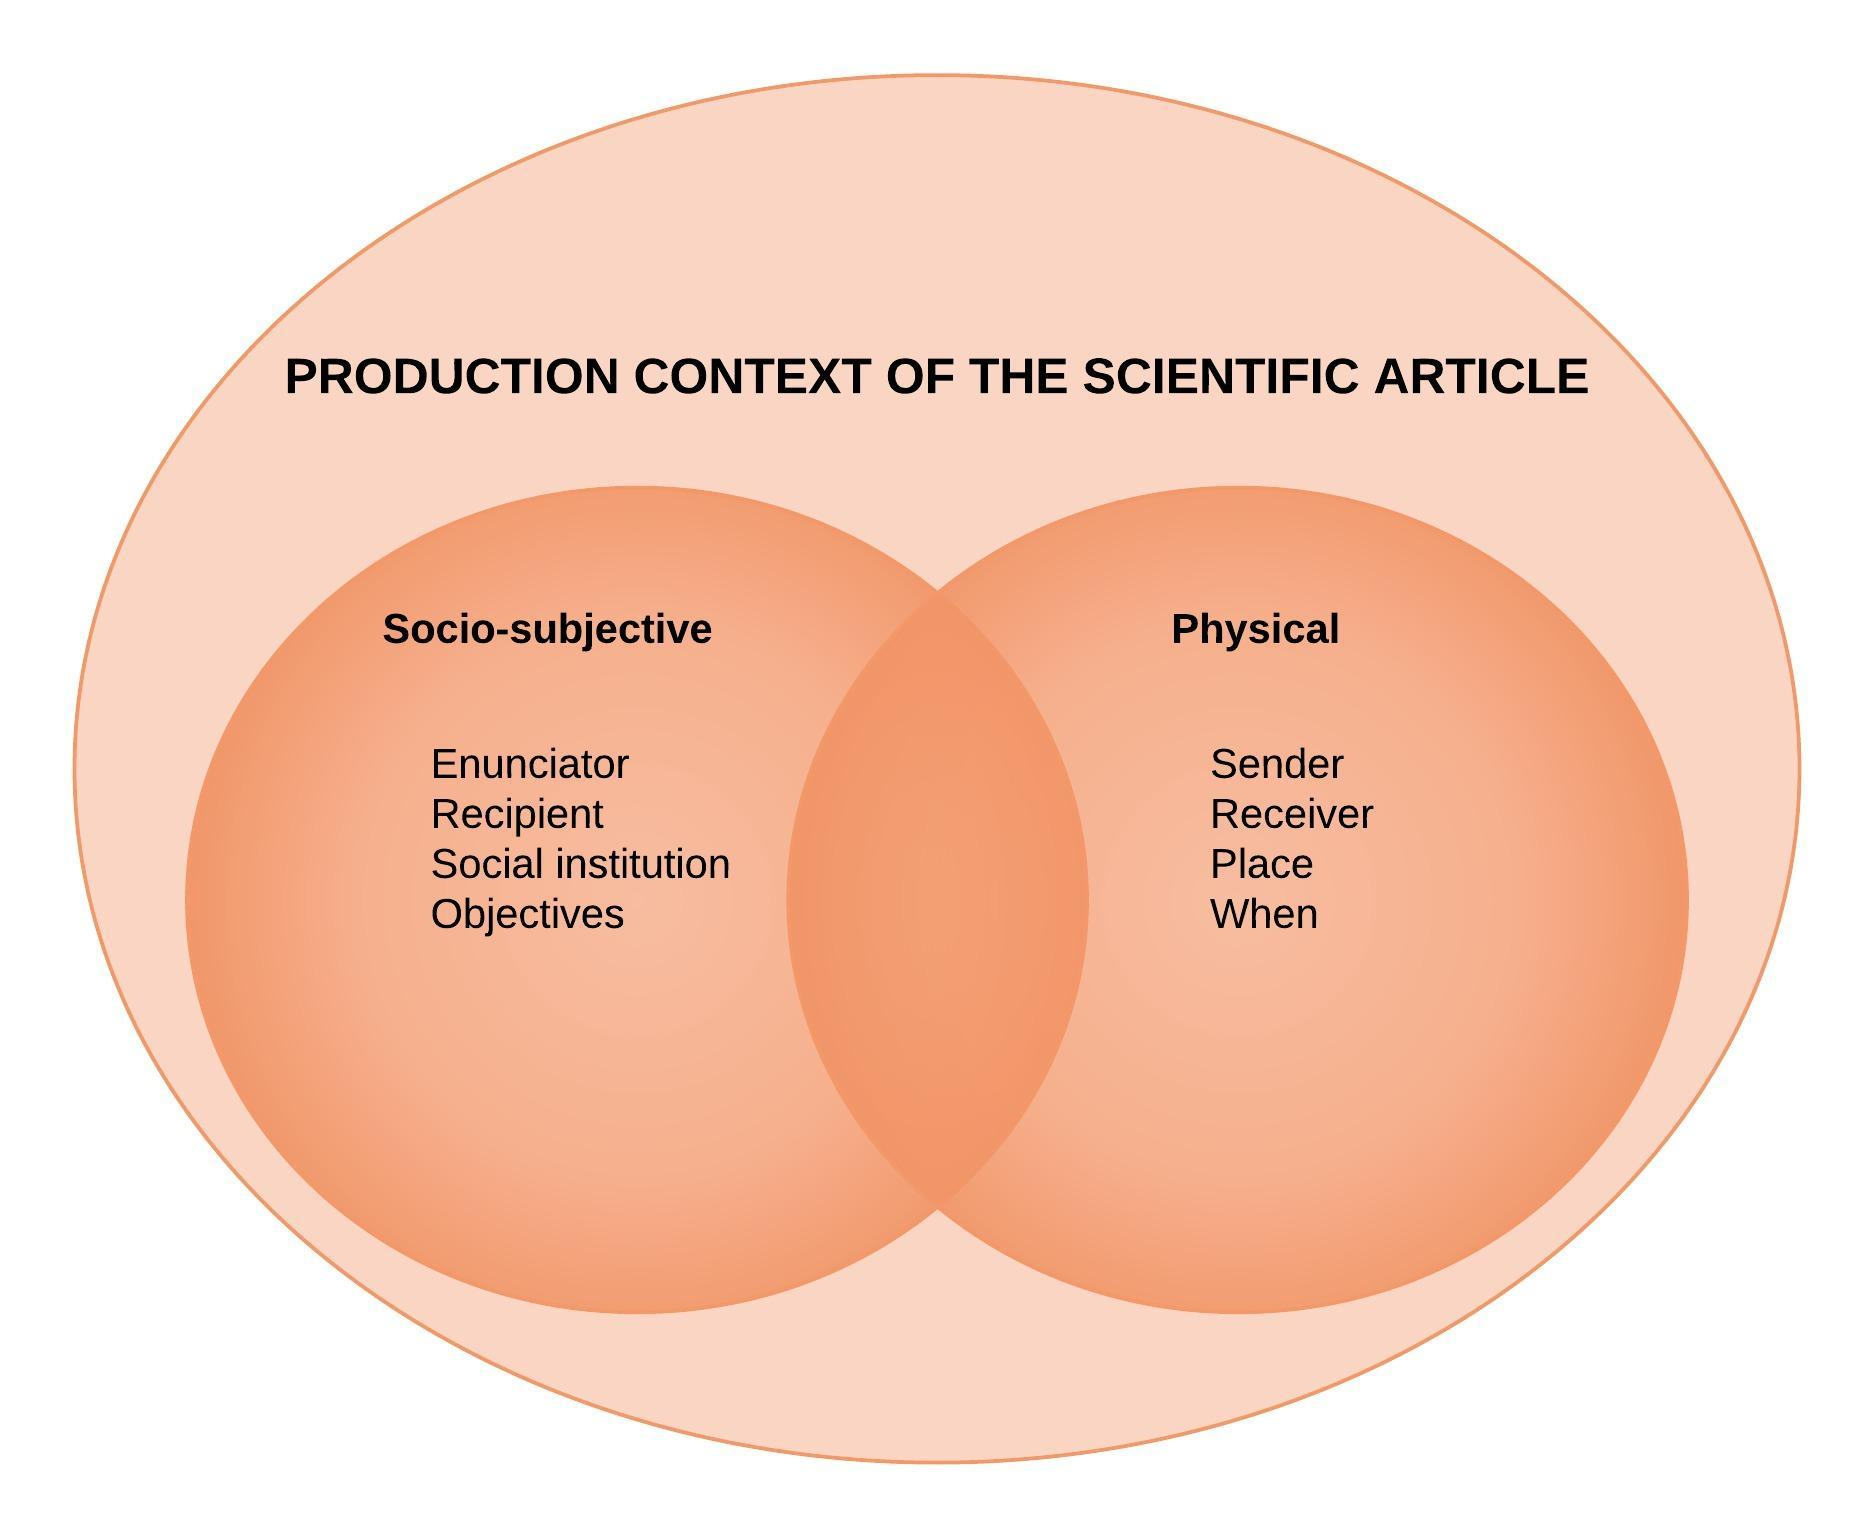
\includegraphics[width=0.85\textwidth]{Fig1.png}
 \caption{Planning the production context of the scientific article.}
 \label{fig-01}
 \source{Adapted from \textcite{bronckart_atividade_1999} model of text analysis.}
\end{figure}

The first level of textual infrastructure is the deepest and is composed of the general plan, which refers to the organization of the set of thematic content. In this context, \textcite[p. 97/98]{bronckart_atividade_1999} considers that it is knowledge that varies according to the agent’s experience and level of development and is previously stored and organized in his or her memory, before the onset of language. Thus, the thematic content of a text consists of the representations constructed by the text’s agent-producer, based on the physical and real world and also on its socio-subjective world. Furthermore, the place and social role the producer assumes must be considered, as well as the historical moment the content is produced and the social position of the recipient. For example, the general plan of a scientific paper is usually comprised of: introduction, theoretical framework, methodology, results and conclusions, and each of these sections has its own specific content and objective.

Some of the main characteristics of the text are compositional structure and text style, since its audience is a group of experts in the field, who are knowledgeable in the subject, familiar with the methodology and interested in the research being developed. These characteristics are decisive in building the text, i.e., the superstructure of the scientific article, as well as the lexical selection of syntactic structures, in other words, the style composition. 

Then, in \Cref{fig-02}, besides presenting the composition of the article’s general infrastructure, a planning model presents an analysis of the second organizational level of the scientific article regarding the style composition, i.e., linguistic-discursive capacities.

\begin{figure}[htbp]
 \centering
 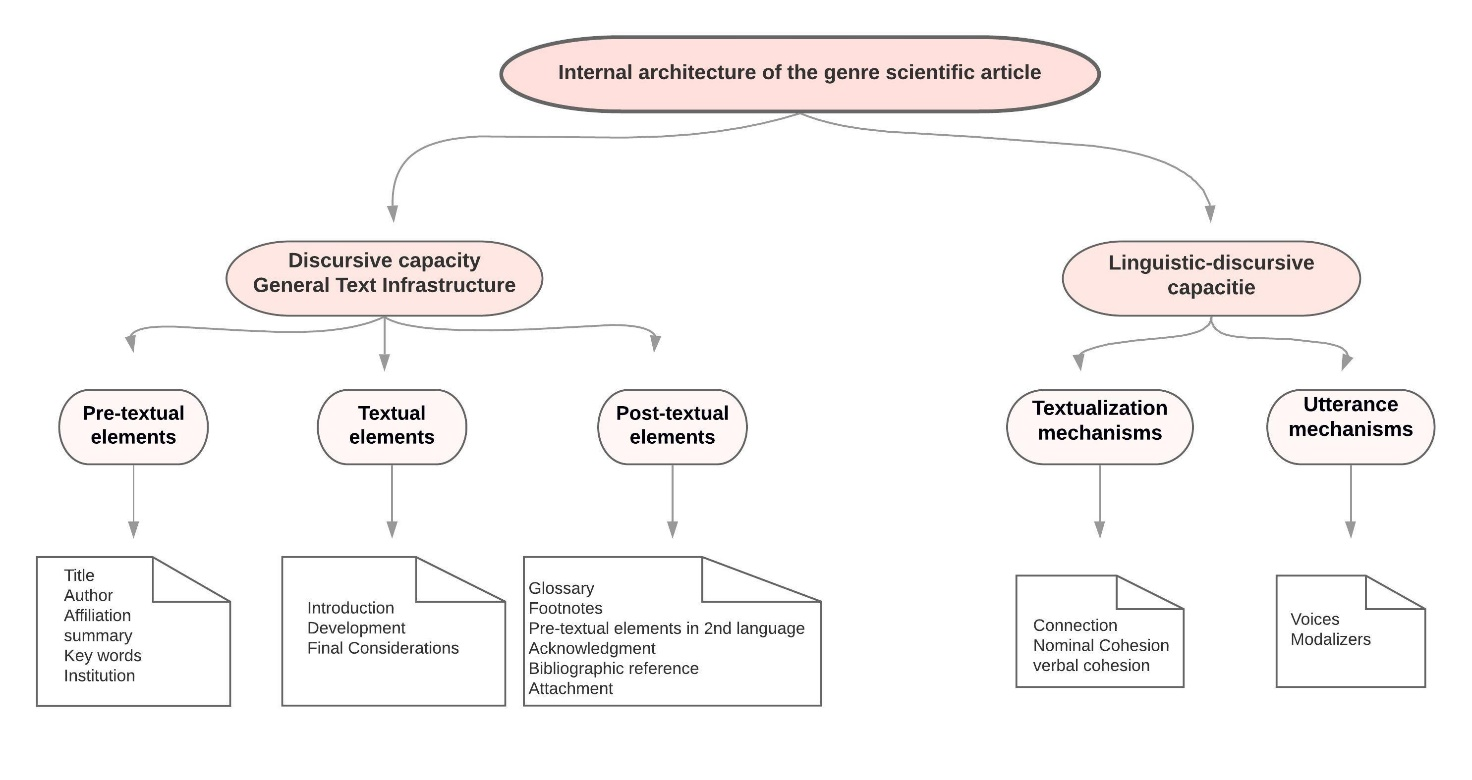
\includegraphics[width=\textwidth]{Fig2.png}
 \caption{Superstructure of the scientific article.}
 \label{fig-02}
 \source{Adapted from \textcite{bronckart_atividade_1999} model of text analysis.}
\end{figure}

The organization of the scientific article’s superstructure represents the second organizational level and refers to textual mechanisms, which are then divided into textualization mechanisms and utterance mechanisms. The purpose of these mechanisms is to contribute to render linear or thematic coherence to the text by elucidating hierarchical, logical, temporal and spatial articulations.

Textualization mechanisms ensure connection, nominal and verbal cohesion. As for utterance mechanisms, the latter ensure progression of the “thematic content”; they refer to the voices assumed within the text and the evaluative mode that composes the utterance. \textcite{bronckart_atividade_1999} states that:

\begin{quote}
    However diverse and heterogeneous the infrastructure components of an empirical text are, it constitutes a coherent whole, a communicative unit, articulated with a situation of action and intended to be understood and interpreted as such by its recipients. This general coherence comes from (...) textualization mechanisms and (...) utterance mechanisms \cite[p. 259]{bronckart_atividade_1999}.
\end{quote}

According to \textcite{silva_elaboracao_2014}, many researchers, such as \textcite{schneuwly_generos_2004}, adopt \textcite{bronckart_atividade_1999} model for didactic purposes and it should be highlighted that this didactic model is required before the genre is taken to the classroom. However, the authors point out that there is a wide range of mechanisms that guide the creation of this model, which are summarized as the three principles of legitimacy, pertinence and solidarity. Again according to the authors, these principles related to the ability of recognizing textual infrastructure and textualization mechanisms can be used as subsidies for the creation of a didactic model of the scientific article genre to support professors and postgraduate students in the development of activities to appropriate this genre.

As in post-graduate courses, these principles related to the ability to recognize textual infrastructure and textualization mechanisms can assist the creation of a representative model of the scientific article genre in order to subsidize applications in automatic text processing through the creation of markups that recover the characteristics which are unique to this genre.

\subsubsection{Organization of representation in the scientific article markup language}\label{sec-organizacao-latex}
\Cref{fig-03} demonstrated the tree-shaped structural model, with XML markups of the main constitutive elements of the representation of the superstructure of the scientific article, which can influence information storage, organization and retrieval in the genre’s automatic processing:  

\begin{figure}[htbp]
 \centering
 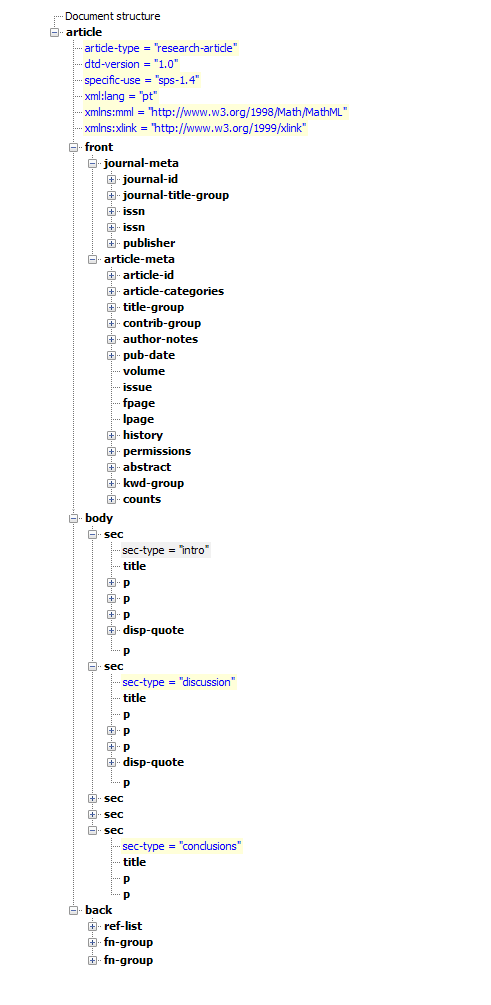
\includegraphics[width=0.5\textwidth]{Fig3.png}
 \caption{Tree-shaped structural model of the main constitutive elements of the scientific article superstructure.}
 \label{fig-03}
 \source{Adapted by the author from the SciELO database.}
\end{figure}

It is possible to observe, through \Cref{fig-03}, that the basic structure of the scientific article genre is represented by the root node (\texttt{<article>}). The root node has as affiliation three more nodes, representative of pre-textual elements (\texttt{<front>}), textual elements (\texttt{<body>}) and post-textual elements (\texttt{<back>}). The pre-textual elements of the \texttt{<front>} characterize and describe the metadata of the journal, title, authorship, affiliation, abstract, key words, DOI, volume, number, supplement, page number, indication of \textit{Creative Commons} license, publication date, header section, date history, correspondence information, author’s notes, book review information, element count and funding data (if any). The textual elements of the \texttt{<body>} characterize and describe the textual body of the article that can be composed of sections. Each one of them possesses an element \texttt{<title>} followed by one or more paragraphs \texttt{<p>}. First level sections can be qualified according to its type through attribute @sec-type, whose possible values, according to the Guia de uso de elementos e atributos XML para documentos que seguem a implementação SciELO Publishing Schema (2016) (\textit{Guide to Using XML Elements and Attributes for Documents Following the SciELO Publishing Schema Implementation}), are the constants from \Cref{tbl02}.

\begin{table}[htbp]
\begin{center}
\caption{Type of Section.}
\label{tbl02}
\begin{tabular}{ll}
\hline 
\textbf{Value}        & \textbf{Description}                                    \\
\hline
Cases        & Cases/case studies                             \\
Conclusions  & Conclusions/final considerations/final remarks \\
Discussion   & Discussions                                    \\
Introduction & Introduction/synopsis                          \\
Materials    & Materials used                                 \\
Methods      & Methodology /methods                           \\
Results      & Results                                        \\ \hline
\end{tabular}
\end{center}
\source{User guide of XML elements and attributes for documents that follow the SciELO Publishing Schema \cite{Scielo}.}
\end{table}

The <back> post-textual elements characterize and describe the final part of the document, comprising the list of bibliographic reference and other research data such as footnotes, acknowledgments, appendix, supplementary material, attachments and glossary.

The representation of the tree-shaped didactic model of the scientific article adds information to linguistic raw data about the characteristics and the visualization of the genre’s constitutive dimensions. It also permits the delimitation of the goals that should be reached regarding different purposes in automatic text processing. As well as \textit{corpus} enrichment with information on the genre composition, in the form of tree-shaped representations, which indicate the relation between elements of the production context (node constants \texttt{<front> <article-meta> </article-meta> </front>}) or sentences or sentence fragments of the general text infrastructure that may apply any structural formalism imposed by the XML source (comprised in \texttt{<body> <sec> </sec> </body>} and \texttt{<back> <ref-list> </ref-list> </back>}) assigned to the genre. This configuration, which consists of converting plain text into structured text, indicates the main genre characteristics that can be used in computational linguistic applications, that is, in automatic preprocessing to solve a given problem or to assist in a given activity for information location, storage and/or retrieval.

This study believes that, from the representative structure of a given text genre, it is possible to organize and prepare the process for receiving and interpreting certain contents for automatic text processing. The preprocessing of a genre will somehow be influenced by the recognition of the superstructure and infrastructure of its compositional organization.

Therefore, the creation and availability of treebanks that can represent language resources constitutive of the text genre is crucial for stimulating a wide range of NLP applications. This structured information is thus important because it indicates the production context and some central textual organizers that may prove to be good preprocessing strategies. Moreover, they constitute databases from which qualitative and quantitative analyzes can be performed using several techniques that may later complement other approaches. 

\subsection{Correlated studies}\label{sec-titulo}
Some textual annotators, which are available for analysis, use a complex approach to categorize data resources and correspondence exploration. Among them, the most popular are: the \textit{morphosyntactic} approach, which specifies how element groups should be organized; and the \textit{semantic} approach, which specifies what the element group should mean. The following computational tools, which use morphosyntactic and semantic approaches for annotation and word processing will be presented below: eDictor, Aelius and COMEDI.

\subsubsection{eDictor}\label{sec-autores}

EDictor\footnote{Available in: \url{https://humanidadesdigitais.org/edictor}. Accessed on: April 19, 2018.} is a tool used to assist electronic XML editing of ancient texts with the purpose of philological analysis and automatic language coding \cite{sousa_o_2014}. This tool was created by the Tycho Brahe\footnote{Available in: \url{http://www.tycho.iel.unicamp.br/corpus/}. Accessed on: April 19, 2018.} Corpus (TBC) annotated for Portuguese, whose main features are: I) flexibility of the generated formats, allowing both human reading and machine reading; II) philological quality assurance due to the fact that it is a specialized editor; III) possibility of operating with several editing levels; IV) Merger, Segmentation, Spelling, Modernization, Expansion, Correction, Punctuation; V) possibility of creating new levels of editing according to the researcher’s needs.

Among its various editing levels, its main features are merging and segmenting. The former is used to merge passages of the text as broken words, while the latter, conversely, separates improperly joined passages. This editing is conducted with XML annotation so it maintains the original text available for reference. These text edits may include other levels of work such as modernization, expansion, spelling and punctuation \cite{sousa_o_2014, sousa_e-dictor:_2010, sousa_uma_2016}.
Dentre seus vários níveis de edição, destacam-se suas principais funcionalidades que são: junção e segmentação. A primeira é utilizada para unir trechos do texto como palavras quebradas, enquanto a segunda faz o oposto, separa trechos indevidamente unidos. Tais edições são feitas com anotação XML de forma a manter o texto original disponível para consulta. Essas edições nos textos podem incluir outros níveis de trabalho como modernização, expansão, grafia e pontuação \cite{sousa_o_2014, sousa_e-dictor:_2010, sousa_uma_2016}.

\subsubsection{Aelius}\label{sec-idioma}
The Aelius\footnote{Available in: \url{http://aelius.sourceforge.net/}. Accessed on April 19, 2018.} software is of free use and under development for superficial analysis of Brazilian Portuguese, which is part of the project Aelius Brazilian Portuguese POSTagger\footnote{Available in: Aelius Brazilian Portuguese Post-tagger - \url{http://sourceforge.net/projects/aelius/files/}. Accessed on April 19, 2018.} and registered with SourceForge.net\footnote{Available in: Sourceforge.Net - Largest Open Source applications and software directory. \url{http://sourceforge.net/}. Accessed on April 19, 2018.} \cite{alencar_aelius:_2010, alencar_aelius_2013a, alencar_aelius_2013b}. Because its architecture is hybrid, the software relies on approaches based on manually formulated rules and on the n-gram-based stochastic statistical system. Aelius has been designed to morphologically and automatically tag written texts. To this end, this editor performs the following tasks: I) corpora preprocessing; II) construction of language models and taggers based on an annotated corpus; III) performance evaluation of a labeler; IV) comparison between different text annotations; V) performing corpora annotation and assisting in human review of automatic annotation.

This tool also includes language features such as language models, sample texts, and gold standards\footnote{In NLP, gold standard means that the strongest and most significant assessments are based on real world results in which a system is operationally deployed and its impact on results generated by real world users is measured \cite{reiter_structured_2018}.}. Aelius currently offers corpora resources and POS corporation and generates annotations in different formats, such as XML in the TEI\footnote{Text Encoding and Interchange (TEI) defines a vast set of elements and attributes in the XML language that allows the representation of structural and conceptual characteristics and text visualization.}P5 encoding scheme.

\subsubsection{COMEDI}\label{sec-resumo}
COmponent Metadata EDItor (COMEDI)\footnote{Available in: \url{http://clarino.uib.no/comedi/page?page-id=repository-main-page}. Accessed on April 19, 2018.} is a web-based component editor for metadata that conforms to any CMDI profile\footnote{Component Meta Data Infrastructure (CMDI) provides a structure for describing and reusing a set of metadata. Available in: \url{https://www.clarin.eu/content/component-metadata}. Accessed on April 19, 2018.} and provides up-to-date support for features implemented by CLARIN\footnote{Common Language Resources and Technology Infrastructure (CLARIN) is a research infrastructure that was launched with the view that all digital language resources and tools throughout Europe and beyond are accessible through an online community using a single logon for supporting researchers in the field of humanities and social sciences. Available in: \url{https://www.clarin.eu/}. Accessed on April 19, 2018.}. With COMEDI, you can create a metadata record from scratch, or upload, edit, and download any CMDI XML file. Its components can be used independently from the editor, or they can be used through a web interface, in which the user selects a CMDI profile to launch and the editor displays the profile as a simple online form that hides the XML code. In addition, the editor can function as a complete server for storing, searching and viewing metadata, as well as exercising control over access rights to individual metadata through group and user administration. The editor’s user administration occurs through login authentication and operates at two levels: user and group \cite{lyse_comedi:_2015}.

The CMDI profile consists of \textit{components} and \textit{elements}. Elements are endpoints, where they are assigned a value, typed in the form body text or selected from a drop-down menu. The elements that belong to endpoints are usually grouped into components; for instance, a person component (with elements such as surname and given name) or a license component (with elements such as license name and license URL). In summary, the recommended profiles, which are found in the COMEDI drop-down menu, are: I) \textit{corpusProfile}: describes the \textit{corpora} of all types and modalities; II) \textit{lexicalProfile}:  describes lexical resources; III) the user is free to develop his or her own profile, but in this case should reuse existing components as far as possible. These recommendations are intended to assist in the description of language resources with metadata according to the CMDI framework. In order to do this, the editor must distinguish required fields from optional fields and make sure required fields are filled out \cite{dima_metadata_2012}.

The computational tools eDictor, Aelius and COMEDI are used for annotation and text processing, based on the use of morphosyntactic and semantic approaches. However, the use of textual genre as a data resource to be explored for annotation and text processing was not observed in the analyzed annotators, revealing the need for a discursive approach.

This article then presents a computational model that uses a discursive approach to filter and categorize the contextual data resources of the scientific article referring to its compositional construction, thus demonstrating the relevance of this kind of annotation for understanding and classifying the genre’s context of production patterns. According to \textcite{cambria_jumping_2014}, recent studies recognize the need to categorize language resources that express external knowledge of the text when interpreting and responding to language input. This knowledge is related to the \textit{pragmatic} approach that specifies how contextual information can be harnessed to provide a better correlation between different existing approaches (morphosyntactic and semantic) and combining them.

\section{Computational model – AnoTex}\label{sec-secoes}
AnoTex\footnote{AnoTex – for automatic corpus construction from the base text genre. Computation tool, Version 0.1 Beta, command line, written in ANSI C, developed to work in any system that uses libc, contains a library for information extraction available in XML and PDF formats, as well as available services for consultation and extension \cite{fonseca_2018}.} is a text annotation tool that is currently under development and whose main purpose is to extract constitutive characteristics from the scientific article by means of XML markers improved with linguistic information about its compositional structure (FONSECA et al., 2018). Its main task is to process the elements of the production context and the general infrastructure of the text for the compilation of the corpus. This tool is able to filter and export annotated elements in XML and its related PDF, extracted from web-based databases such as \textit{SciELO-Scientific Electronic Library Online}.\footnote{Available in: \url{http://www.scielo.br}. Accessed on Jan 12, 2018.}.

The set of applications developed by AnoTex is demonstrated in \Cref{fig-04}, which, in short, corresponds to the design of the computational model that adequately attends the research goals, divided into four steps, namely: 1 selection, 2 compilation, 3 processing and 4 data export.

\begin{figure}[htbp]
 \centering
 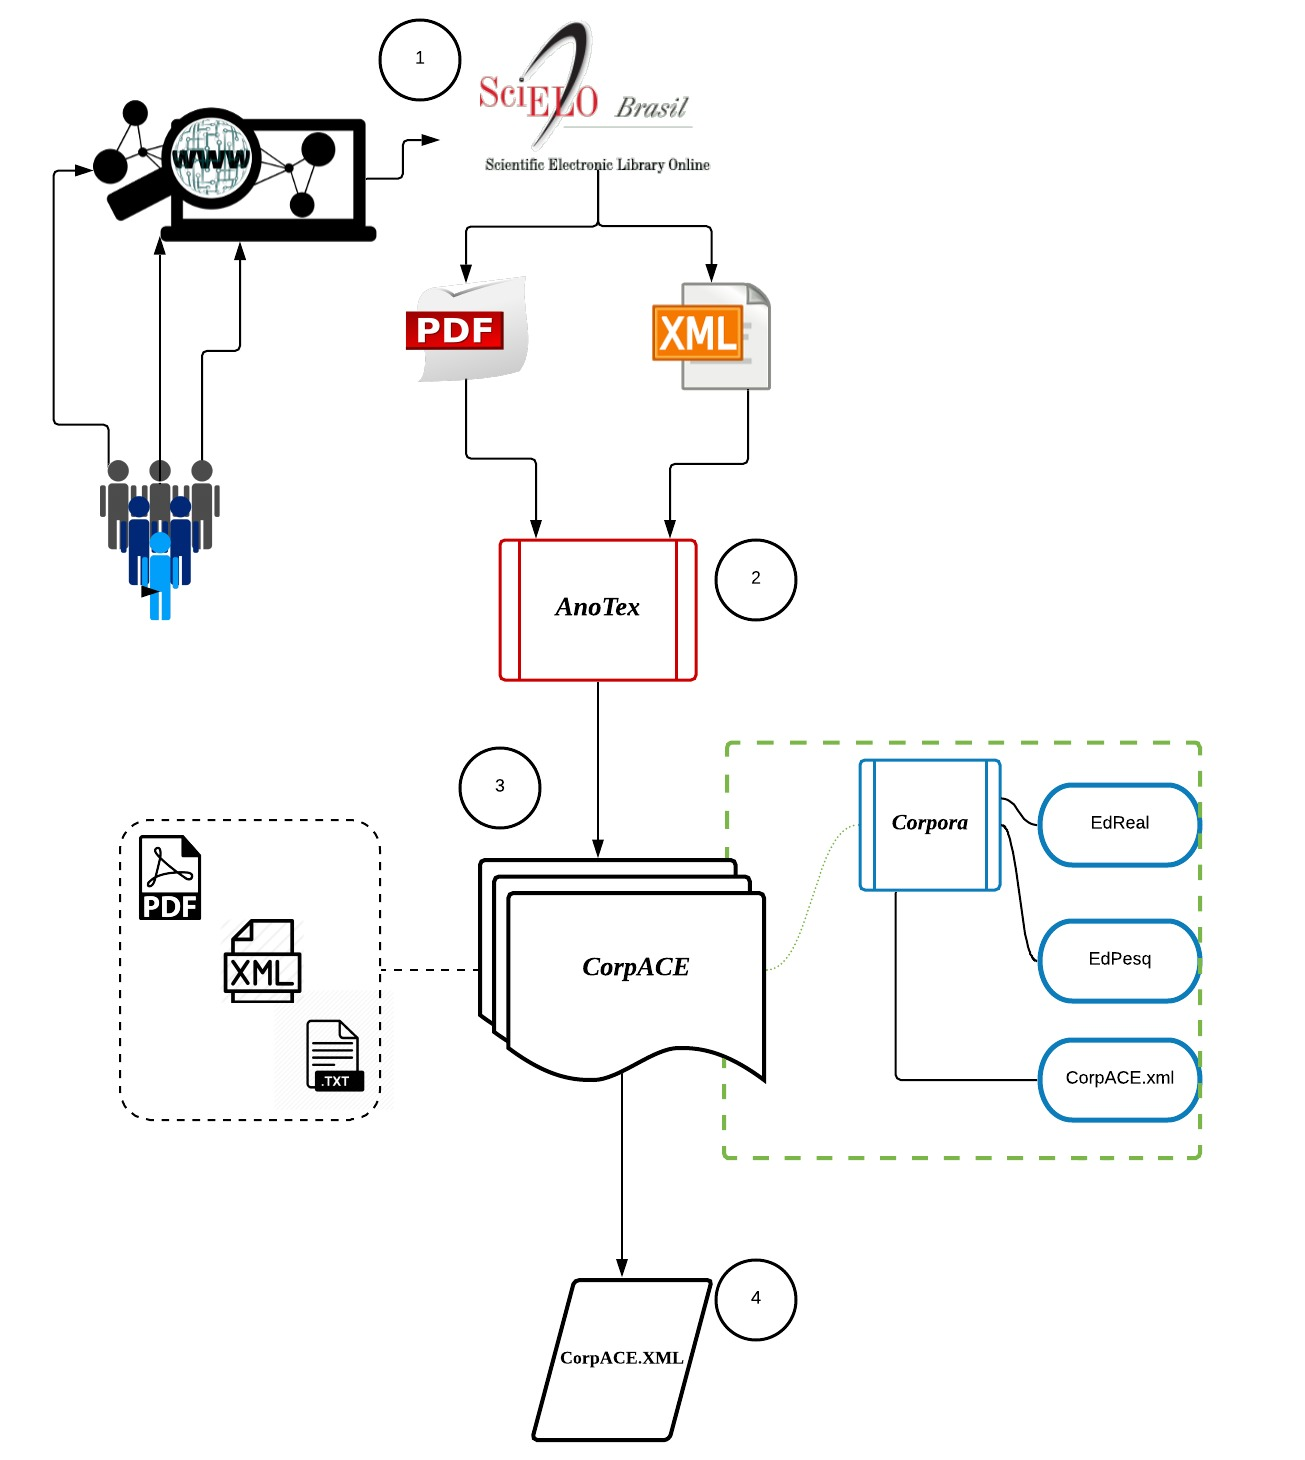
\includegraphics[width=0.85\textwidth]{Fig4.png}
 \caption{AnoTex Compilation Model.}
 \label{fig-04}
 \source{\cite{fonseca_etal_2018}.}
\end{figure}

The first three steps illustrated in the model concern data quality, namely:

\begin{enumerate}
    \item \textit{Selection}:a set of requirements of the genre is selected, highlighted by the use of XML tags, which is necessary to impact the validity and reliability of the analyzed corpus, adapting it to the research purposes, thus allowing it to underline the traits and the visualization of the constitutive dimensions of the scientific article;
    \item \textit{Compilation}: the set or sample of genre constitutive data is collected for manipulation; in other words, it is at this stage that the corpus which will compose the corpora for analysis is organized and generated;
    \item \textit{Processing}: transformation and/or treatment of data like noise, inconsistencies, missing or incomplete data, which can generate distorted patterns; elimination of redundant attributes, standardization of the value set of selected elements from the articles.
The AnoTex currently filters 06 pre-textual elements, included in the \texttt{<front>} through categorization and markup with information on: \textbf{Journal title}: \texttt{<journal-title> </journal-title>}; \textbf{Article title}: \texttt{<article-title> </article-title>}; \textbf{Author name}: \texttt{<contrib contrib-type="author"> <name> <surname> </surname> <given-names> </given-names> </name>}; \textbf{Institution}: \texttt{<institution content-type=""> </institution>}; \textbf{Abstract}: \texttt{<abstract> <title></title> </abstract>}; \textbf{Key words}: \texttt{<kwd-group xml:lang=""> <title> </title> <kwd></kwd> </kwd-group>}.
  
Within the textual elements, included in the \texttt{<body>}, sections and subsections are filtered through categorization and markup with information on: \textbf{Introduction}: \texttt{<sec sec-type="intro"> <title></title> </sec>}; \textbf{Discussion}: \texttt{<sec sec-type="discussion"><title></title></sec>}; \textbf{Conclusions}: \texttt{<sec sec-type="conclusions"><title></title></sec>}.

In addition, AnoTex filters the bibliographic references of post-textual elements, comprised of \texttt{<back>} with categorization and tagging with information on: \textbf{Bibliographic References}: \texttt{<ref-list> <title> </title> <ref> </ref> </ref-list>};
    \item \textit{Export}: Serializes the corpus into a XML file, for interpretation and evaluation of the patterns identified according to the initial objectives. These steps converge to form a concise database in which data from different journals is collected and stored in a single data set.
\end{enumerate}

\Cref{fig-05} below shows a sample of the CorpACE configuration generated by AnoTex. The pre-textual elements shown in 1, 2, 3, 4 5, 8 and 10 correspond to the representation of the production context; the textual elements demonstrated in 6 and 9 correspond to the representation of the general text architecture, as well as the post-textual elements shown in 7.

\begin{figure}[htbp]
 \centering
 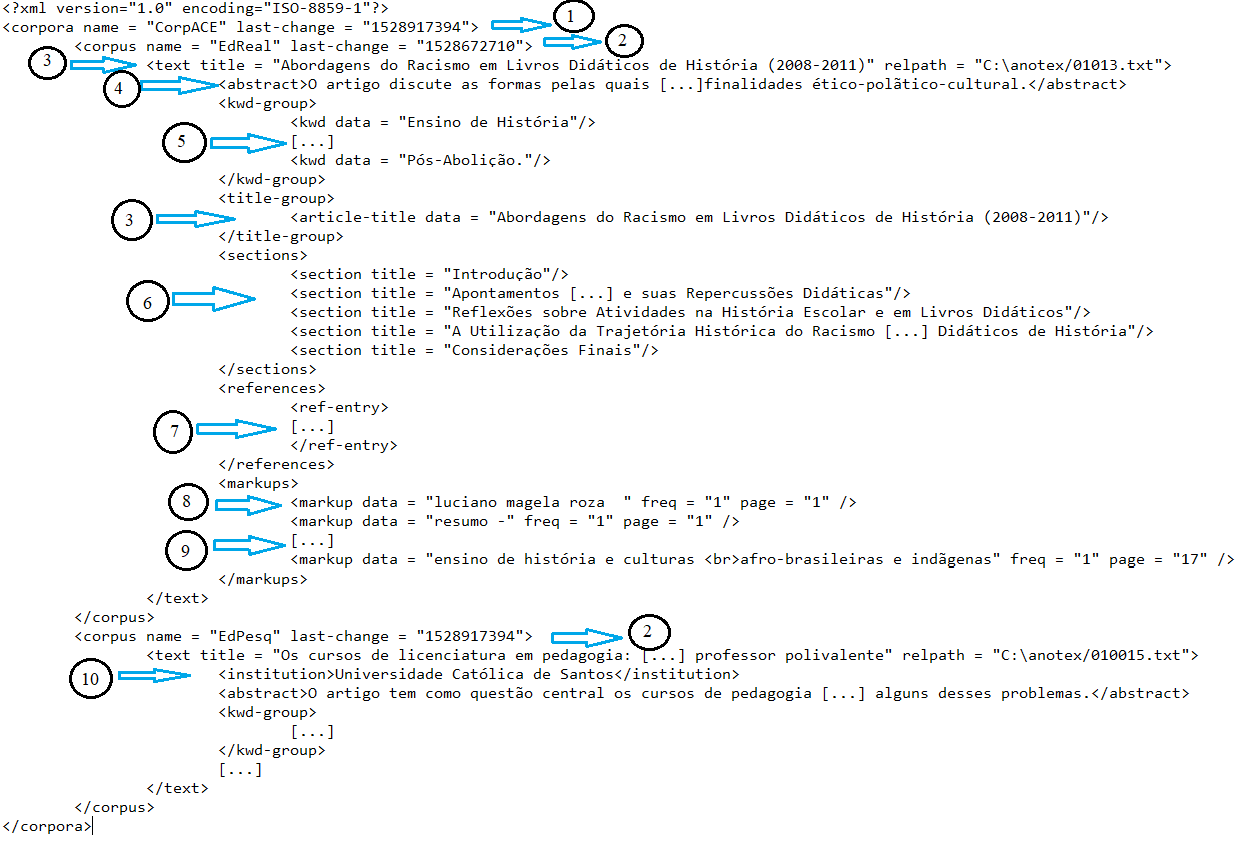
\includegraphics[width=\textwidth]{Fig5.png}
 \caption{Sample of the \textit{CorpACE} configuration.}
 \label{fig-05}
 \source{Adapted by the author from AnoTex v0.1b.}
\end{figure}

Through \Cref{fig-05}, it is possible to observe that, after filtering each element, AnoTex creates a \textit{CorpACE} generating an output XML file (based on XML and PDF data entry). This textual base will be useful for linguistic analysis, training and analysis of computational tools whose purpose is text processing. The separation between structure and data presentation affords malleability of information.

The textual basis will be used for linguistic analysis, training and analysis of computational tools whose purpose is word processing. The separation between data structure and representation renders greater flexibility to information (from the same XML, it is possible to represent the information in different ways in addition to supply metadata for a database). The data represented by XML is tree-structured, and each tag or label represents a node or element in the tree.

For \textit{corpora} output in an XML file, AnoTex had to receive five required arguments: PDF file, XML file, name of corpora, name of output file, and specification of which corpus the markup has been to from this output file. The advantage of this process is that an output XML file can gather multiple \textit{corpora}, a very useful requirement if, for example, one must create different versions of the same \textit{corpus}. AnoTex allows the creation of multiple \textit{corpora}, added within the same file and this requirement set constitutes the \textit{corpora} of the file. All of these features could be viewed in \Cref{fig-04} and \Cref{fig-05}.

\section{Results and discussion}\label{sec-format-simple}
The results of this study are based on 87 scientific articles classified as \textit{Qualis} A1\footnote{\textit{Qualis} is a Brazilian system for journal assessment developed by \href{https://pt.wikipedia.org/wiki/Coordenação_de_Aperfeiçoamento_de_Pessoal_de_Nível_Superior}{CAPES} (Coordination for the Improvement of Higher Education Personnel), a foundation that lists and classifies the media used for publishing the intellectual production of post-graduate programs (Masters and PhD) according to circulation (local, nationwide or international) and quality (A, B, C) by field. The strata are divided into 8 levels, by order of quality.}, published in 2017 by the following journals: \textit{Revista Educação \& Realidade} and \textit{Revista Educação e Pesquisa}\footnote{Available in: \url{http://www.educacaoepesquisa.fe.usp.br/}. Accessed on Jan 12, 2018.}. The articles were retrieved from the SciELO website and recorded in individual files in PDF, XML and TXT formats, which are supported by AnoTex. The compilation of these files generated the CorpACE, which is characterized as specialized corpora, since it is composed by texts from a single area of expertise – educational, and representative of a single text genre – scientific article. According to the scheme by \textcite{sardinha_linguistica_2004}, regarding extent, the corpora is classified as medium-sized. \Cref{tbl03} is presented below with the main numerical data that characterize CorpACE:

\begin{table}[htbp]
\begin{center}
\caption{Statistical Results of \textit{CorpACE}.}
\label{tbl03}
\begin{tabular}{ll}
 \toprule 
\textbf{Statistics}         &        \textbf{Total} \\ \hline                          
Number of articles         &         87                              \\
Total word count   &                 750380                          \\
Word count of smallest article    &  6144                            \\
Word count of largest article  &     18758                           \\
Average word count per article          &         8625               \\
Word count filtered from constitutive elements of genre    &   130128 \\
Word count of \textit{Corpus} EdReal     &  383506                             \\
Word count of \textit{Corpus} EdPesq   &     366874                            \\ \hline 
\end{tabular}
\end{center}
\source{Created by the author.}
\end{table}

\textit{CorpACE} underwent computational treatment through CL, which is methodologically present in this research by means of the AnoTex tool that generated the data from \Cref{tbl03}. Two main libraries of the tool were used for filtering XML and PDF data from the article files. The first one was used to organize the \textit{corpora} into a treebank with information on the production context and the general text infrastructure. The second one was used to obtain data from expressions in bold and italics with statistical information about location and the frequency in which they appeared in the texts. The tool helped organize data and analyze the elements which most often appeared in scientific articles.

\textit{CorpACE} is made up of three sets of \textit{corpora}, with a total of 750,380 words, distributed in 87 scientific articles. These \textit{corpora} are subdivided as follows: corpus EdReal (Revista Educação e Realidade), with 383,505 words distributed within 45 scientific articles; \textit{corpus} EdPesq (Revista Educação e Pesquisa), with 366,874 words distributed within 42 scientific articles; and CorpACE.xml with 130,128 words from filtered elements (FE) from 87 articles.

The first step consisted of analyzing the collected data in the XML file generated in the output of AnoTex and then organizing and systematizing the result of the genre markup constituent elements that were selected and specified in processing step 3.

Subsequently, after delimiting each \textit{corpus}, this study presented the count and systematization of the EdReal and EdPesq \textit{corpora} separately, according to filtered element, in \Cref{fig-06}:

\begin{figure}[htbp]
 \centering
 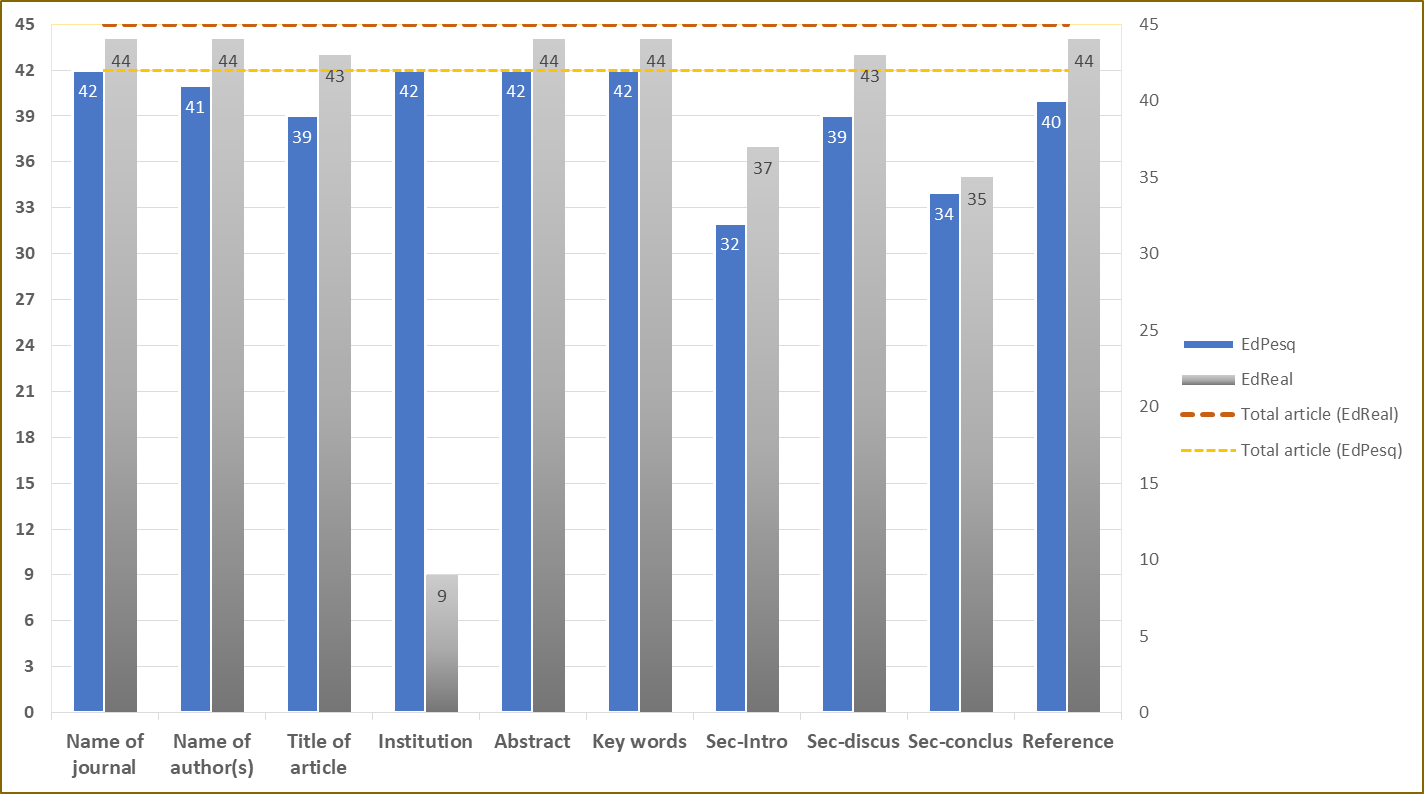
\includegraphics[width=0.85\textwidth]{Fig6.png}
 \caption{Filtered elements by \textit{corpus}.}
 \label{fig-06}
 \source{Created by the author.}
\end{figure}

\Cref{fig-06} shows the number of elements that were filtered from scientific articles of each corpus. The results indicate that the AnoTex tool managed to filter the constitutive elements of the genre from the 42 selected articles from the journal Revista EdPesq, in the following proportions:

\begin{itemize}
    \item \textit{Elements of the \texttt{<front>}}: Name of journal 100\%; Name of author(s): 97.6\%; Title of article: 92.9\%; Institution: 100\%; Abstract: 100\%; Key words: 100\%;
    \item \textit{Elements of the \texttt{<body>}}: Introduction section: 76.2\%; Discussion section: 92.9\%; Conclusion section: 81.0\%;
    \item \textit{Elements of the \texttt{<back>}}: Reference: 95.2\%.
The element filtering, which is constitutive of the genre of the 45 articles selected from EdReal Magazine, was as follows:
    \item \textit{Elements of the \texttt{<front>}}: Name of journal 100\%; Name of Author(s): 100; Title of Article: 97.8\%; Institution: 20.0\%; Abstract: 97.8\%; Key words: 97.8\%;
    \item \textit{Elements of the \texttt{<body>}}: Introduction section: 82.2\%; Discussion section: 95.6\%; Conclusion section: 77.8\%;
    \item \textit{Elements of the \texttt{<back>}}: Reference: 97.8\%.
\end{itemize}

The result of the filtered element Institution \texttt{<institution content-type=""> </institution>} was noteworthy because of the discrepancy between elements filtered by the journal \textit{Revista EdReal} and those by \textit{Revista EdPesq}. The shift occurred due to a tagging problem in the markup tag \texttt{<aff id="aff1">}, by the journal, as there was a loose "I" in the middle of the code, which confused the AnoTex parsing. In order to fix this problem, the "I" was wrapped with the markup \texttt{<label> I</label>}, also marked in other files that worked, thus solving the problem and allowing for data filtering (\Cref{fig-07} and \Cref{fig-08}).

\begin{figure}[htbp]
 \centering
 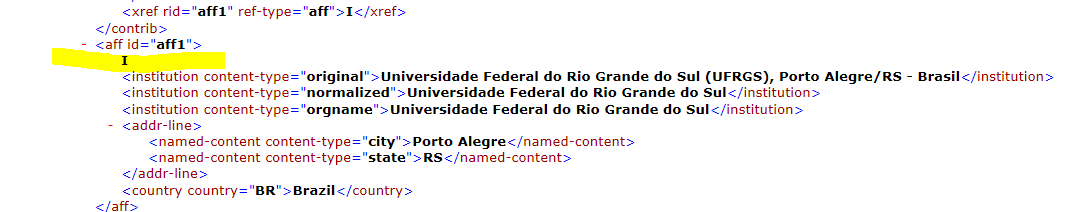
\includegraphics[width=\textwidth]{Fig7.png}
 \caption{Representation of the code with a marker problem.}
 \label{fig-07}
 \source{Adapted by the author from \textit{CorpACE}.}
\end{figure}

\begin{figure}[htbp]
 \centering
 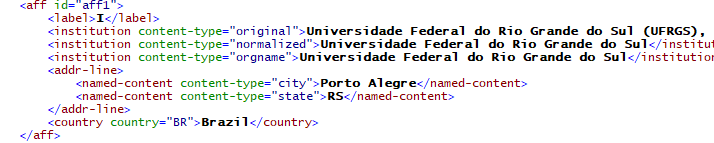
\includegraphics[width=0.85\textwidth]{Fig8.png}
 \caption{Representation of the code without problems and after corrections.}
 \label{fig-08}
 \source{Adapted by the author from \textit{CorpACE}.}
\end{figure}

Although this discrepancy occurred in filtering the <institution> element, due to a problem in XML production, the overall result was considered satisfactory, as shown in \Cref{fig-09}:

\begin{figure}[htbp]
 \centering
 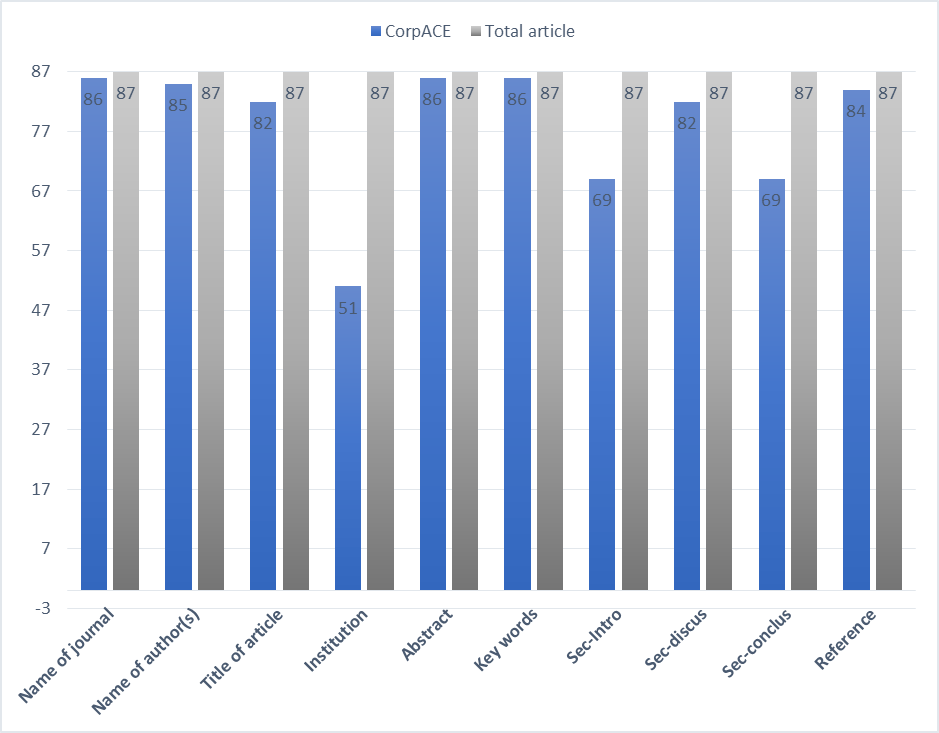
\includegraphics[width=0.85\textwidth]{Fig9.png}
 \caption{Total elements filtered for \textit{CorpACE}.}
 \label{fig-09}
 \source{Created by the author.}
\end{figure}

\Cref{fig-09} shows the total number of elements that have been filtered from scientific articles. The results indicate that the AnoTex tool was able to filter at least 4 and at most 10 representative elements of the genre in all 87 selected articles, in the following proportions:

\begin{itemize}
    \item \textit{Elements of the <front>}: Name of journal: 100\%; Name of author(s): 98.9\%; Title of Article: 95.4\%; Institution: 58.6\%; Abstract: 98.9\%; Key words: 98.9\%;
    \item \textit{Elements of the <body>}: Introduction section: 79.3\%; Discussion section: 94.3\%; Conclusion section: 79.3\%;
    \item \textit{Elements of the <back>}: Reference: 96,6\%.
\end{itemize}

Still regarding the analysis of distortions, another noteworthy element was the markup of the title of the article \texttt{<article-title> </article-title>}. Although all the markings with this denomination had been filtered, we consider for the result only the one that brought the tag and the content of the text (the title itself). Out of 87 analyzed files, 04 had been filtered by the tag \texttt{</article-title>}, but the title of the text had not. They were replaced by the expression (null) instead of the title information. It was observed that, in these four samples, the titles were represented with different characters – partly in bold or as a footnote, for example. The file included a tag that confounded the filtering logic. According to the AnoTex logic, as more than one tag was found, a new indirection was created. Thus, the title was located at a level below where it should.

Normally, when following the recommendations of the SciELO publication guidelines, the relevant title data itself is at the level labeled "article-title" as shown in \Cref{fig10}.

\begin{figure}[htbp]
 \centering
 
\includegraphics[width=\textwidth]{Fig10.png}
 \caption{Representation Title.}
 \label{fig10}
 \source{Adapted by the author from \textit{CorpACE}.}
\end{figure}

With the variation of the "bold" markup, the title became “article-title->bold->"o título"”. \Cref{fig-11} illustrates the mentioned variation:

\begin{figure}[htbp]
 \centering
 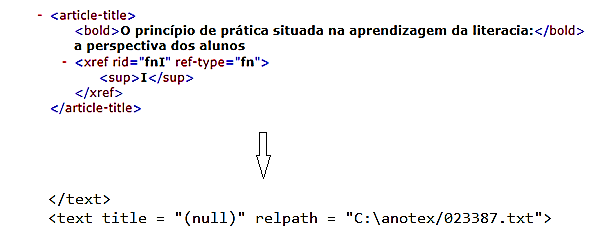
\includegraphics[width=0.85\textwidth]{Fig11.png}
 \caption{Title located below where it should.}
 \label{fig-11}
 \source{Adapted by the author from \textit{CorpACE}.}
\end{figure}

This file shows a distinct discrepancy between the journal’s annotation and the recommendations contained in the  SciELO Guidelines \citeyear{Scielo}. In that case, a lot of information was concentrated where there should only have been a single direct and valuable piece of information: the title described in the format we humans would refer to the article. Since these markups are conducted by professionals working for the Journal, this demonstrates that the title should go through a normalization stage before being tagged, as it would allow greater use of the available language resources. To specifically address this issue, a change was made to this variation so that if AnoTex finds the tag “bold”, it should ignore it. In the illustrated case, the bold tag (\texttt{<bold>} and \texttt{</bold>}) was removed and the title was re-filtered.

Another feature revealing a slight disparity in annotation was the filtered data for Sec-intro (introduction section), Sec-discus (discussion section), Sec-conclu (conclusion section) elements. Although there are specific recommendations in the Guideline regarding XML elements and attributes for documents that adhere to the \textit{SciELO Publishing Schema}, Version 1.5.1 \citeyear{Scielo}, as shown in \Cref{tbl02} - Type of Sections, the articles do not follow a strict standard and homogeneous format for the body of text markup, <body>. Therefore, the results of this study only considered articles that had sections with the attribute \texttt{<sec-type>} (\Cref{fig-12}).

\begin{figure}[htbp]
 \centering
 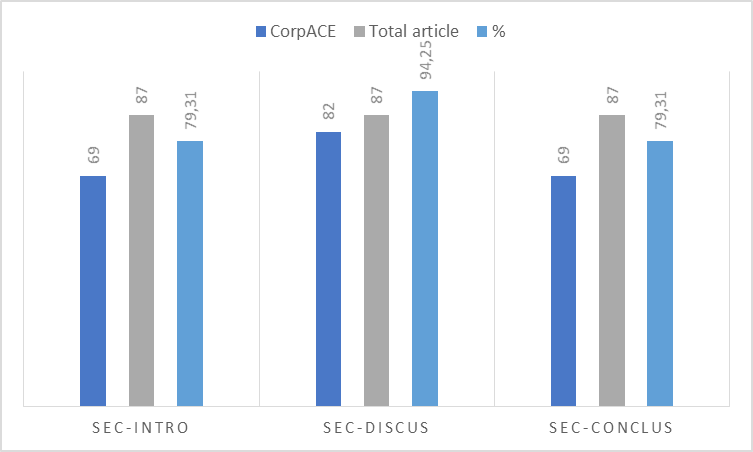
\includegraphics[width=0.85\textwidth]{Fig12.png}
 \caption{Filtering section elements.}
 \label{fig-12}
 \source{Created by the author.}
\end{figure}

Following this specification, the results showed that, in one of the analyzed samples, one of the articles was unmarked for the section attribute. In other samples, the markups for this attribute did not comply with the standards recommended by the Guideline. When these elements were filtered out, it was observed that, sometimes, sections in the article’s first level presented the attribute <sec-type> defined by the SciELO Guideline as: \texttt{<sec sec-type="intro">}, with 69 occurrences; \texttt{<sec sec-type="discussion">} with 82 occurrences; and \texttt{<sec sec-type = "conclusions">} with 69 occurrences; sometimes they only showed the <sec> attribute without specifying the type, with 17 occurrences; and one time there were no markups and the entire text of the article was marked only by paragraphs (this was observed in only one sample). This finding made it possible to understand that the data markup system does not require the existence of the attribute \textit{sec/@sec-type}; i.e., it is not a mandatory recommendation for journals.

While this study analyzed, in practice, the use of XML markups in article sections for text processing with NLP tools, it also verified a few issues that confused the AnoTex parsing logic. In an analyzed sample, for instance, a first-level section that matches a list of nearby values necessarily presented an \textit{@sec-type} attribute and the Discussion and Conclusion sections, which are from the first level, were contained within the also first-level Introduction section. In this case, since the guideline does not recommend this type of markup, AnoTex did not predict the markup variation, so the tool was unable to filter out the sections that were nested within the <sec sec-type="intro">.  To explain this case, two hypotheses were raised: there could have been an error in XML production, or the discussion and conclusion sections would be directly dependent on the first introduction section and, for that reason, there were no other sections in the text. However, the Guide does not address this type of markup.

These types of variations, albeit few in number, reveal that that academic journals should start applying a stricter and more homogeneous standard in XML representation so that they can be more efficiently “tracked” online and processed by computational tools. Aside from being more useful and more semantic, markups would become easier if standardization were more pervasive. However, this reality is still far from being applied due to the enormous variation in format and data represented in the articles. Furthermore, for the SciELO standard alone, there are 8 different versions, from Version 1.1 to Version 1.8, which lead to tags piling up. Coding schemes must evolve in order to meet new demands so as not to break compatibility with older versions of programs, and programs need to be prepared to handle older versions of data for backward compatibility.

This is not always easy to apply in practice, for artificial languages follow a standard that arises from development and technological implementation and they are extremely context-sensitive. On the other hand, natural languages, before being represented/transformed by XML tags, for example, must be understood and normalized. The authors realized that there are several forms of representing the same language resource, which, in some cases, may not favor interaction compatibility.

Although the study came across some variations that confused the parsing logic, an analysis of most of the collected data revealed that, among the elements that can be filtered by AnoTex, and which made up \textit{CorpACE}, a basic structure of the scientific article genre can be highlighted, consisting of pre-textual (\texttt{<front>}), textual (\texttt{<body>}) and post-textual (\texttt{<back>}) elements. This rigid structure observed in most of the 87 collected articles derives precisely from the base text function, which must be elaborated according to the journals’ pre-established norms, and for its intended purpose, in order to assure scientific communication of the subject addressed. This confirms the assumption that the structure of the analyzed genre is conditioned to its social function.

XML markups enhanced with linguistic information about the compositional construction of the genre, in the form of tree representations that indicate the relationships between elements of the production context (node constants \texttt{<front> <article-meta> </article-meta> </front>}), or sentences or sentence fragments of the general text infrastructure (comprised in \texttt{<body> <sec> </sec> </body>} and \texttt{<back> <ref-list> </ref-list> </back>}), allow the transformation of plain text into structured text. Through this representation, from the same XML, it is possible to reuse, present information in different ways, and indicate the main characteristics of the genre that can be used in computational linguistic applications.

These tags that were filtered, compiled, and exported by the AnoTex computational tool generated an output file in XML format. One of the advantages revealed by this type of output file configuration was the creation of a corpus that could be used by a larger number of tools in such a way as to serve a variety of purposes and following, as a rule, the data provided by SciELO XML file. Furthermore, the separation between the structure and presentation of the collected elements will render greater flexibility to the corpus, because through this configuration it is possible to present the data in different ways, as well as to load metadata into a database.

Another important point that should be discussed is that each element that composes the corpus includes a relative path (relpath). In this case, the corpus is composed by a main XML file ('CorpACE.xml') and a sub-folder ('texts') containing the whole text in txt. This path is important because, in automatic text processing, when a tool reads a section <text> ... </text>, it will know exactly where to find the corresponding full text using this procedure. This functionality is demonstrated by the arrows in \Cref{fig-13} below:

\begin{figure}[htbp]
 \centering
 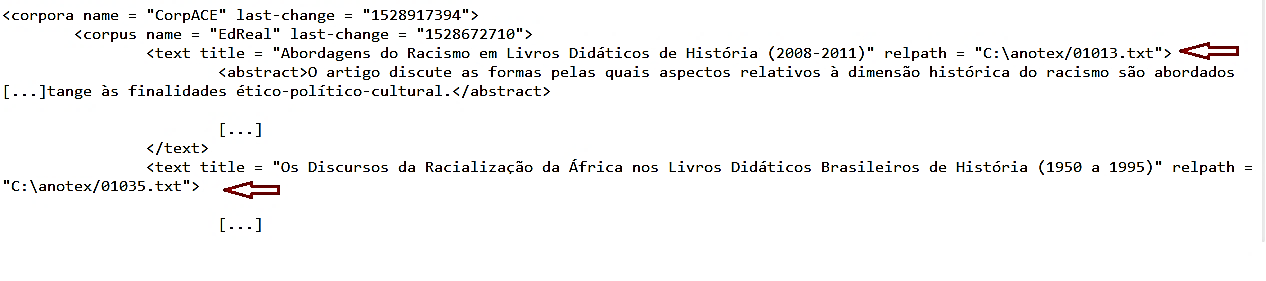
\includegraphics[width=\textwidth]{Fig13.png}
 \caption{Relative Path for Text Location.}
 \label{fig-13}
 \source{Adapted by the author from AnoTex v0.1b.}
\end{figure}

The analysis of the collected data confirmed the initial hypothesis of the research – the scientific article structure is contingent upon its social function, since are linguistic events characterized by a set of communicative purposes and by being relatively stable types of utterances. XML markings of representations of aspects related to the \textit{context of production} of the scientific article can influence the way the text is organized. The filtered elements constituting these markings reveal: sender/enunciator, receiver /recipient, place/institution, support and thematic content. Regarding the genre’s \textit{general architecture}, which is related to text content management – the compositional construction characteristic of the genre, AnoTex initially filters the discursive capacities of the genre comprehended in three subdivisions, characterized in Figures 11 - Pre-Textual Elements; 12 - Textual Elements and 13 – Post-Textual Elements, as follows:

\begin{enumerate}
    \item \textit{Pre-textual} Elements in the <front> such as: journal, title, author, institution, abstract, and keywords (\Cref{fig-14}).
\begin{figure}[htbp]
 \centering
 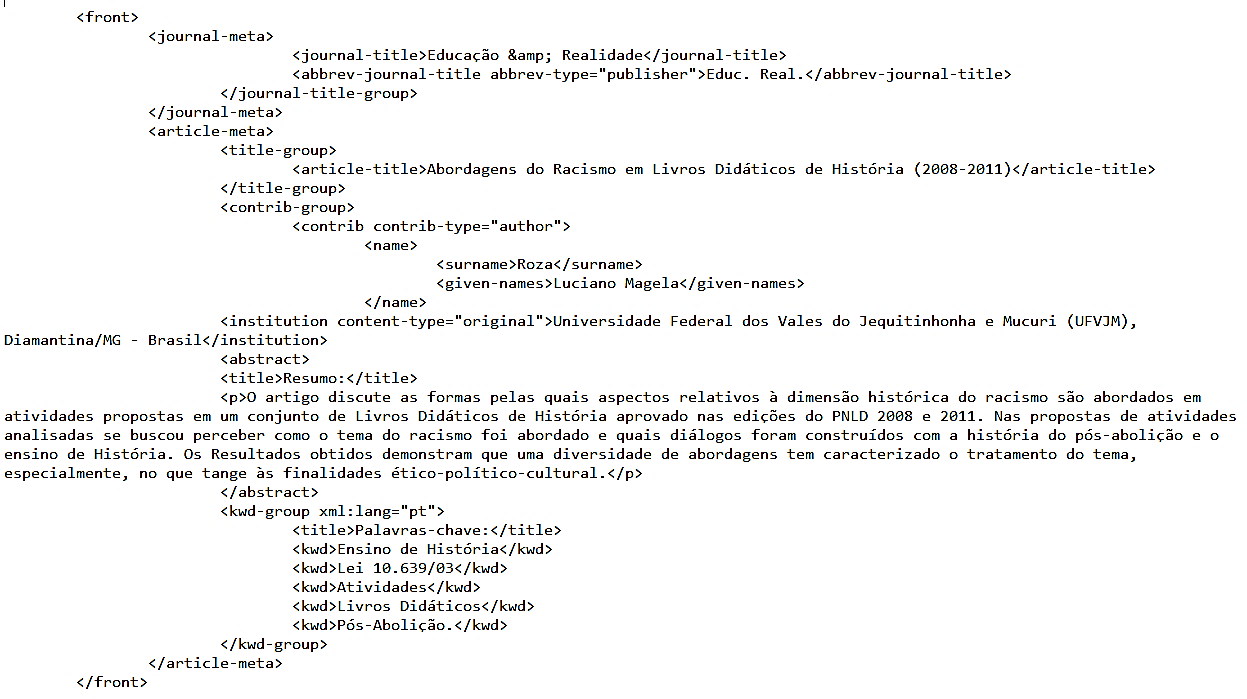
\includegraphics[width=\textwidth]{Fig14.png}
 \caption{Pre-textual Elements.}
 \label{fig-14}
 \source{Adapted by the author from \textit{CorpACE}.}
\end{figure}
    \item \textit{Textual} elements present in the <body> such as: introduction, discussion and final considerations (main sections of the article): (\Cref{fig-15}).
\begin{figure}[htbp]
\centering
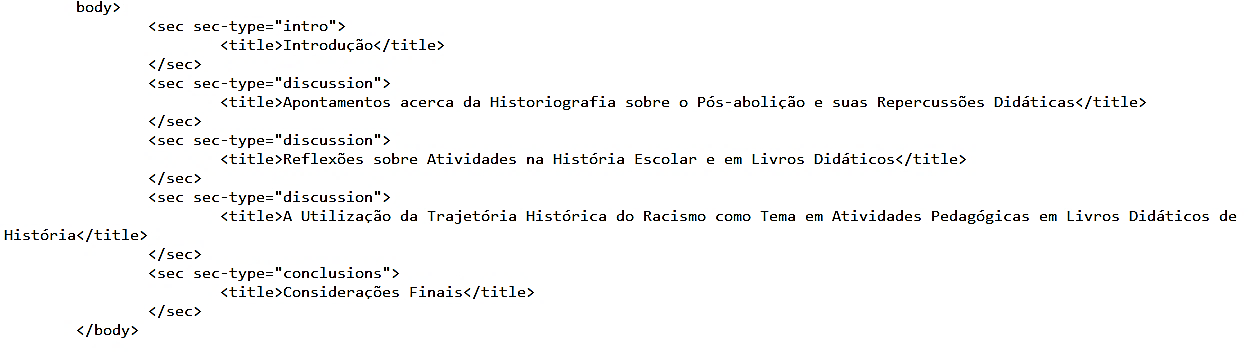
\includegraphics[width=\textwidth]{Fig15.png}
\caption{Textual Elements.}
\label{fig-15}
\source{Adapted by the author from \textit{CorpACE}.}
\end{figure}
    \item \textit{Post-Textual} elements present in the <back> such as: bibliographic references. (\Cref{fig-16}).
\begin{figure}[htbp]
\centering
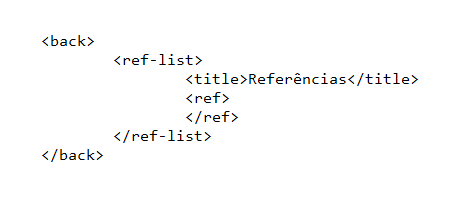
\includegraphics[width=0.85\textwidth]{Fig16.png}
\caption{Post-Textual Elements.}
\label{fig-16}
\source{Adapted by the author from \textit{CorpACE}.}
\end{figure}
\end{enumerate}

%Verificar se há erro no código de figura dentro da enumeração

This configuration of the computational model that represents the scientific article genre, emphasized by the use of XML tags, made it possible to highlight the characteristics and visualization of the constitutive dimensions of the genre, and to delimit different purposes for which it is used. Moreover, this tree representation of the constitutive elements of the corpus may give clues to the characteristics of the genre that can be mined and valued for text processing.

It may become relevant to indicate the location and number of occurrences through bold and italic filters, since the most conclusive and significant elements may appear on pages closer to the introduction (\texttt{<sec sec-type="intro">})  or the conclusion (<sec sec-type = "conclusions">) in scientific articles \cite{lin_identifying_1997}.
%(LIN; HOVY, 1997). 
In this case, through the basic structure of the genre, a weight could be established for the term by observing the page where it occurred, as well as the number of times it was found and marked throughout the article. From a linguistic point of view, this is information that still needs to be explored in the valuation of sentence ranking.

\section{Conclusion}\label{sec-links}
As we analyzed the XML markups (enhanced with linguistic information about the genre’s compositional structure, which indicate the relations between elements of the context of production and/or general infrastructure of the base text) for text processing through NLP tools, we were able to verify, in practice, some aspects that fuzz AnoTex’s parsing logic. However, an analysis of most of the collected data revealed that, among the elements that can be filtered by AnoTex, and which formed the \textit{CorpACE}, a basic structure of the scientific article can be highlighted, composed of pre-textual (\texttt{<front>}), textual (\texttt{<body>}) and post-textual (\texttt{<back>}) elements. The solidness observed in the structure of most of the 87 chosen articles stems precisely from the function of the base text, which is supposed to be elaborated in conformity with pre-established norms required by academic journals and with goals and purposes for which it is designed, as it ensures the representative model of the subject addressed. This ratifies the assumption that the structure of the analyzed genre is contingent upon its social function.

Given the assessment of the currently available corpus annotation tools, it is argued they do not sufficiently describe the traits of the base text genre, in combination with an adequate level of usability. Since the main purpose of these tools’ approach is conducting morphosyntactic and semantic annotation, a gap in the base genre’s structure has been demonstrated. Therefore, it is possible to state that there is a necessity of a closer relationship between the automatic text annotation system and the analysis of the base text genre. And, by means of this approach, AnoTex is able to fill a major gap in the development of applications for identifying and analyzing structured data that is representative of the genre so as to provide new guidelines for the field in terms of processing a large number of texts. Since texts are purposeful communicative events, the decisions regarding its relevant properties imply recognizing the source’s properties, as they are fed by a set of prerequisites with communicative purposes.
 
Another important point that deserved to be highlighted is that coding schemes need to evolve in order to meet new demands so as not to be incompatible with older versions of the programs, and programs must be prepared to deal with older versions of data, enabling backward compatibility. However, natural language, before being represented by/transformed into artificial language, through XML markups for instance, should be understood and normalized, otherwise it may not favor interaction compatibility.

We must make use of technology to address the multiple knowledge areas that are needed in order to improve the linguistic traits of NPL-focused applications, rather than allowing overspecialization. We believe that new studies will be conducted and, among them, there may be a possibility for the unification of different fields of knowledge, rendering communication between men and machine more efficient.

\printbibliography\label{sec-bib}
% if the text is not in Portuguese, it might be necessary to use the code below instead to print the correct ABNT abbreviations [s.n.], [s.l.]
%\begin{portuguese}
%\printbibliography[title={Bibliography}]
%\end{portuguese}


%full list: conceptualization,datacuration,formalanalysis,funding,investigation,methodology,projadm,resources,software,supervision,validation,visualization,writing,review
\begin{contributors}[sec-contributors]
\authorcontribution{Claudia Aparecida Fonseca}[conceptualization,formalanalysis,investigation,methodology,writing,review]
\authorcontribution{Marcus Vinícius Carvalho Guelpeli}[datacuration,formalanalysis,software,projadm,supervision,visualization]
\authorcontribution{Rafael Santiago de Souza Netto}[formalanalysis,software,visualization,writing]
\end{contributors}

\end{document}

